\subsection{Light sources}
In gpvdm light comes from light sources, which are defined in the light source editor which can be found in the Optical ribbon of the main window see figure \ref{fig:opticalribbon}.

\begin{figure}[H]
\centering
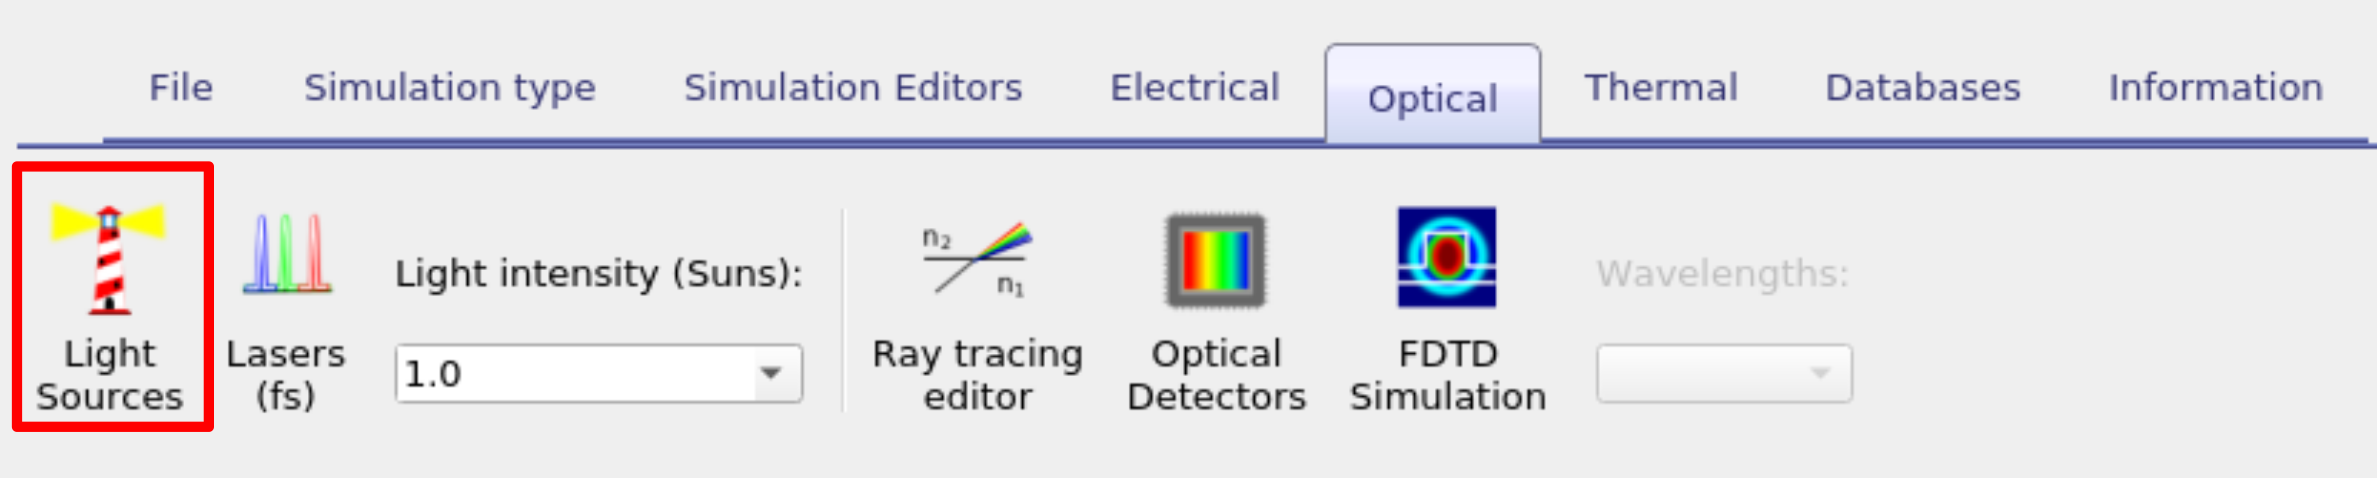
\includegraphics[width=0.7\textwidth]{./images/light_ribbon.png}
\caption{Opening the light source editor.}
\label{fig:opticalribbon}
\end{figure}

The light source editor is shown below in figure \ref{fig:lightsourceeditor}.
\begin{figure}[H]
\centering
\begin{tabular}{ c c }

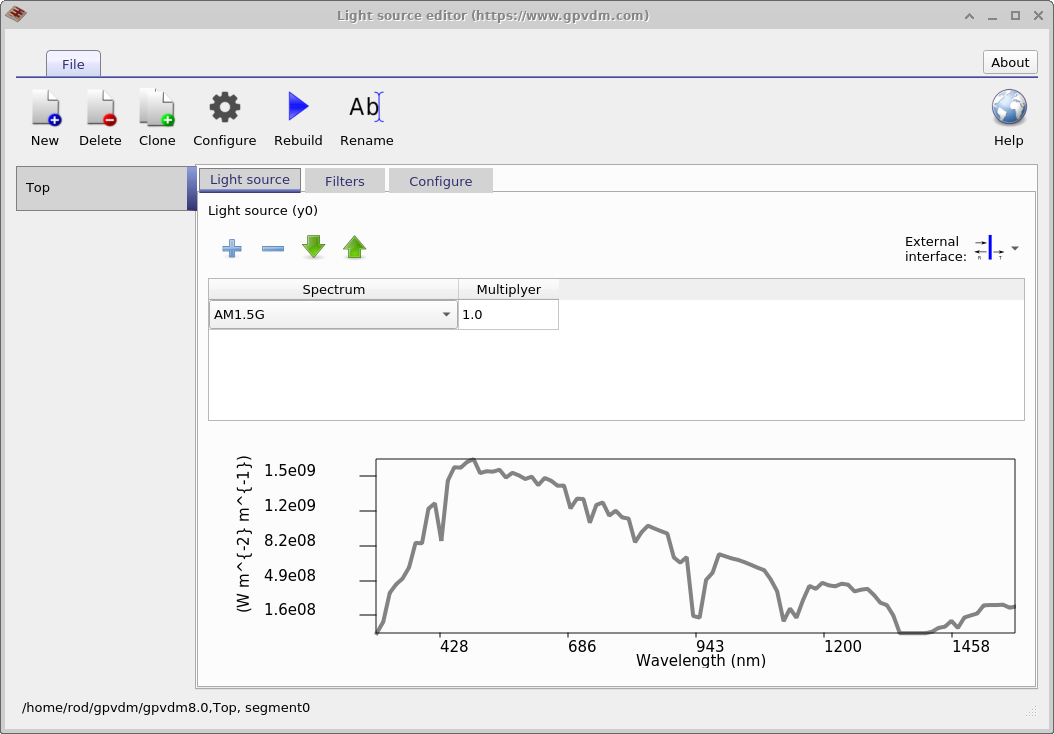
\includegraphics[width=0.5\textwidth,height=0.4\textwidth]{./images/lights0.png}

&
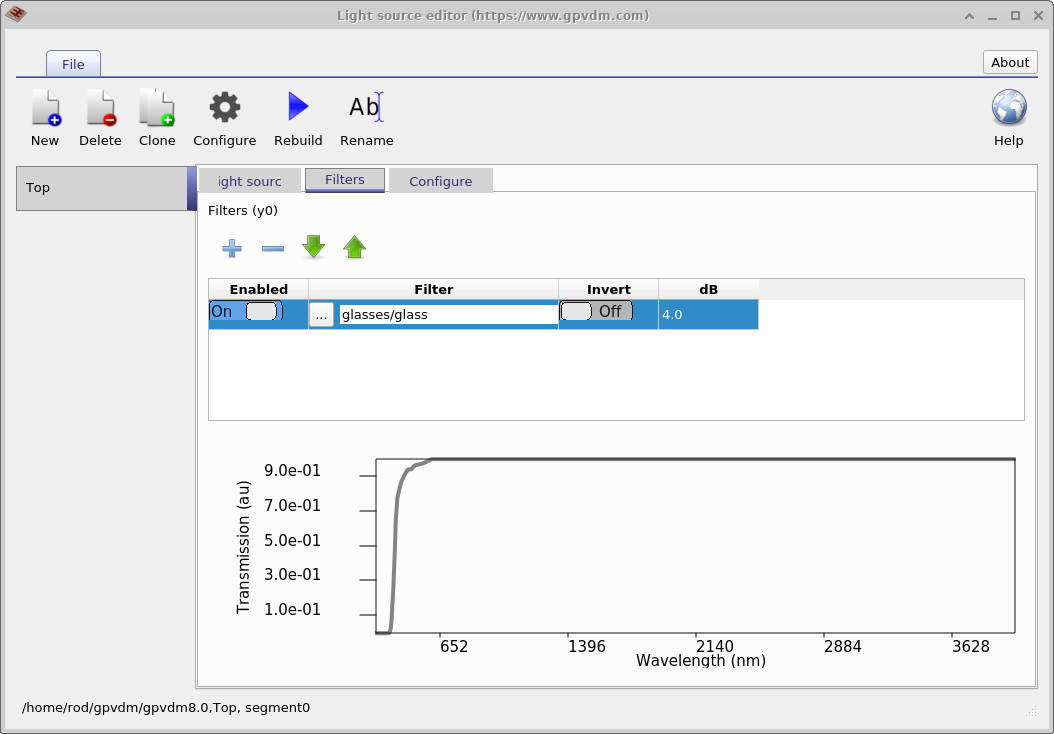
\includegraphics[width=0.5\textwidth,height=0.4\textwidth]{./images/lights1.png}
\\
\end{tabular}
\caption{Left: Building an optical spectrum; Right modifying the light sources with optical filters.}
\end{figure}


\begin{figure}[H]
\centering
\begin{tabular}{ c c }

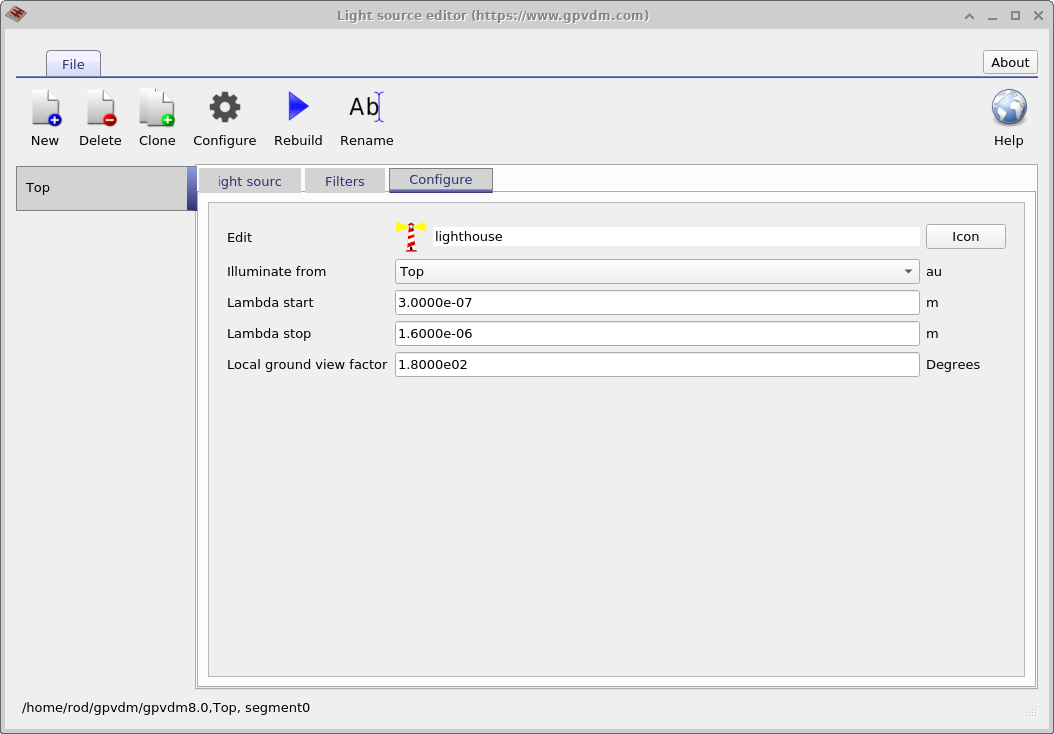
\includegraphics[width=0.5\textwidth,height=0.4\textwidth]{./images/lights2.png}

&
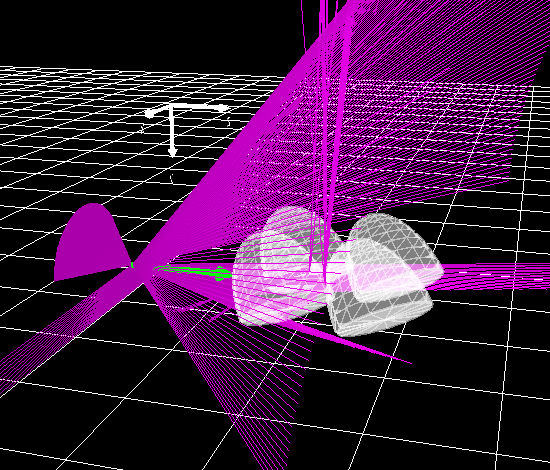
\includegraphics[width=0.5\textwidth,height=0.4\textwidth]{./images/light_xyz.png}
\\

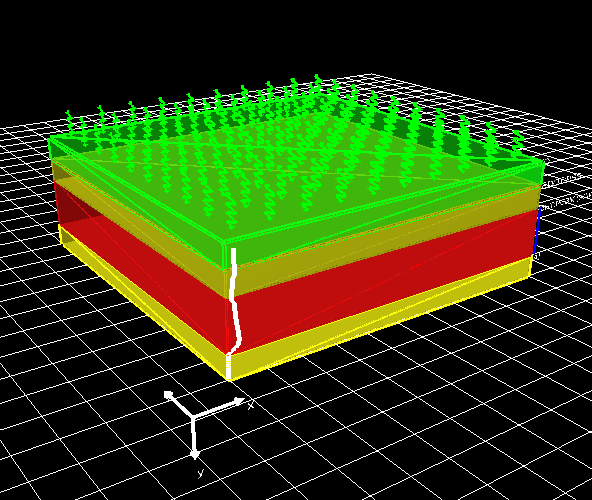
\includegraphics[width=0.5\textwidth,height=0.4\textwidth]{./images/light_top.png}

&
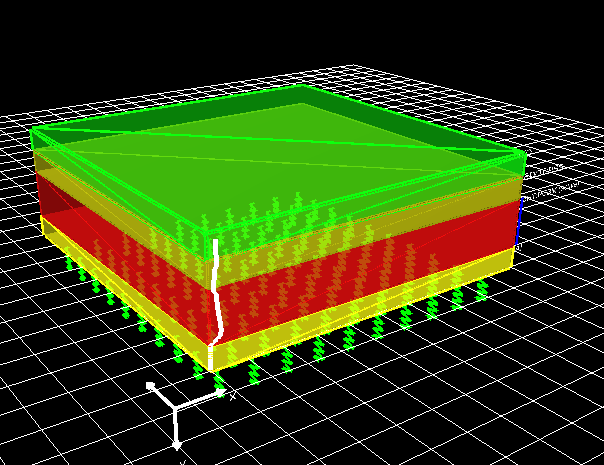
\includegraphics[width=0.5\textwidth,height=0.4\textwidth]{./images/light_btm.png}
\\
\end{tabular}
\caption{Top left: The configure panel of the light source editor; Top right: Illuminate from set to "xyz"; bottom left: Illuminate from set to "top"; bottom right: Illuminate from set to "bottom".}
\label{fig:lightsourceeditor}
\label{fig:transfermatrix1}
\end{figure}



\subsubsection{Local ground view factor}
The local ground view factor is given as \cite{neryterrain}

\begin{equation}
F_{ground}=sin^2 \left ( \frac{\theta_t}{2}\right )=\frac{1-cos(\theta_t)}{2}
\end{equation}

